\documentclass[12pt,a4paper,twoside]{article}
\usepackage{graphicx,fancyhdr}

%\pdfpagebox=4

\setlength{\parindent}{0cm}
\setlength{\parskip}{2ex plus1ex minus 0.5ex}

\addtolength{\evensidemargin}{-2.5cm}
\addtolength{\oddsidemargin}{-0.5cm}
\addtolength{\textwidth}{3cm}

\addtolength{\headheight}{0.2cm}
\addtolength{\topmargin}{-2.5cm}
\addtolength{\textheight}{2.5cm}

% \newcommand{\source}[1]{\textbf{\verb^#1^}}}
\renewcommand{\_}{\texttt{\symbol{95}}}
\addtolength{\fboxsep}{0.1cm}
\newcommand{\param}[1]{\textit{\textrm{\textmd{#1}}}}
\newcommand{\codebar}{\rule{\textwidth}{0.3mm}}
\newcommand{\todo}{\textbf{TODO}}

\newlength{\codelen}
\newcommand{\code}[1]
{\begin{center}\fbox{\parbox{16cm}{\texttt{#1}}}\end{center}}

\newcommand{\mission}[1]{\item[#1:]}
% \newcommand{\mission}[1]{\texttt{#1}\hspace{3mm}}

\fancyhead{}
\fancyhead[RO,LE]{\thepage}
\fancyhead[LO,RE]{Tealight Summer School Projects}
\fancyfoot{}
\pagestyle{fancy}
% \pagestyle{empty}

\setcounter{secnumdepth}{1}

\newenvironment{bulletlist}
{
	\begin{itemize}
	\addtolength{\itemsep}{-1mm}
	% \setlength{\itemsep}{0ex}
	\setlength{\parsep}{0ex}
}
{
	\end{itemize}
}

\newenvironment{alphalist}
{
	\begin{enumerate}
	\setlength{\itemsep}{0ex}
	\setlength{\parsep}{0ex}
	\renewcommand{\labelenumi}{(\alph{enumi})}
}
{
	\end{enumerate}
}

\newenvironment{numericlist}
{
	\begin{enumerate}
	\addtolength{\itemsep}{-1mm}
	% \setlength{\itemsep}{0ex}
	\setlength{\parsep}{0ex}
}
{
	\end{enumerate}
}

\usepackage{hyperref}
\begin{document}

\centerline{\textbf{\LARGE Tealight Summer School Projects}}
\vspace{0.5cm}
\centerline{August 2015}
\centerline{Author: Ian Davies}
\centerline{Based on ROBOC projects by David Eyers (\texttt{David.Eyers@cl.cam.ac.uk})}

{ \parskip 1mm plus 1pt \tableofcontents }

\section*{Introduction}

All projects use Art mode in Tealight.
The most difficult project is Racetrack; all projects are marked with
their approximate difficulty.

\newpage
\section{Paint program \it{(Easy)}}

The aim of this project is to start with the sketch program, and
develop it into a more fully-featured painting program. Start by
adding a colour palette. When the user clicks on the palette, it
should change their drawing colour. Do a three colour palette
first (say black, red and white); then try a larger one. You
should use a loop to draw the larger palette, specifying colours
by number instead of name, to make the program shorter. You can
calculate which colour the user has clicked on from the coordinates,
and turn this into the colour number. You may want to add a display
of the current drawing ink colour. Here is an example palette:

\begin{center}

\includegraphics[scale=0.6,angle=0]{screenshots/artpixel/paint/palette}
\end{center}

Next, try adding a toolbox which lets the user select from different
drawing tools. For example you could let them draw lines, spots, squares,
stars, triangles, or with an italic pen nib. There could be a tool which
draws balloons using the \verb^image^ function. You could consider
different size tools, or an eraser.
Here is an example toolbox, and some different tools in use:
\begin{center}
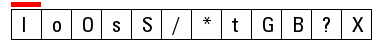
\includegraphics[scale=0.6,angle=0]{screenshots/artpixel/paint/toolbox}\\[2mm]
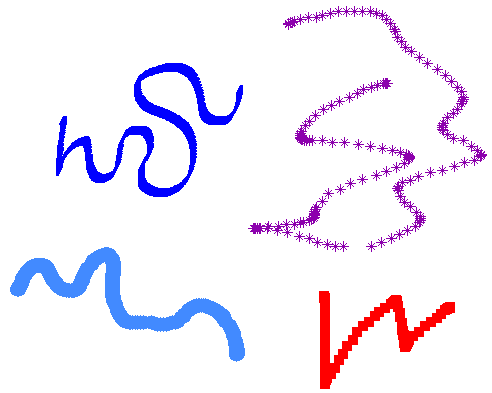
\includegraphics[scale=0.5,angle=0]{screenshots/artpixel/paint/tools}
\end{center}

\subsection{Extension}

Allow two users on different computers to participate
by drawing on the same canvas (so both users see the results of both
drawing on their screen). First use the \verb^send^ command to notify the other
computer when the user has clicked with the mouse. See the Networking section of the user manual for hints.
Initially you might arrange for it to display a shape in the
corner of the screen when the other user clicks with the mouse, just to
test the communication is working. Make it work in both directions.

Next you will need to encode the coordinates where the other user has
clicked within the network message it sends.

\newpage
\section{Memory game \it{(Easy)}}

This project is to write a memory game, in which playing cards (with
pictures of animals) are arranged on the screen. The player clicks
on two cards, which are turned over; if they match they are both removed,
otherwise they are hidden from view again. Play continues until there
are no cards left.

It is advisable to begin with some simpler programming tasks.
Write a function to print 48 playing card backs in a grid, using the
\verb^Card^ image. Then write a function to print 24 pairs of animals
in a grid (2 each). Next, create an array
to hold the card numbers, and work out a way of using the
\verb^random^ function to mix up the order. Display the
48 mixed up animals. Allow the user to click on cards; deduce
which card position has been clicked on and remove it from the
display. Then put this all together to make the game.

The left picture below shows the animals arranged in a grid during testing
(during the game they are never all shown at once, of course), before
the \verb^random^ function has been used to mix them up. The right picture
shows a typical situation during a real game, in which most of the cards
are face down, some pairs have already been removed, and the user has
just turned over two cards (which don't match, so these will be hidden
again next time they click the mouse).

\begin{center}
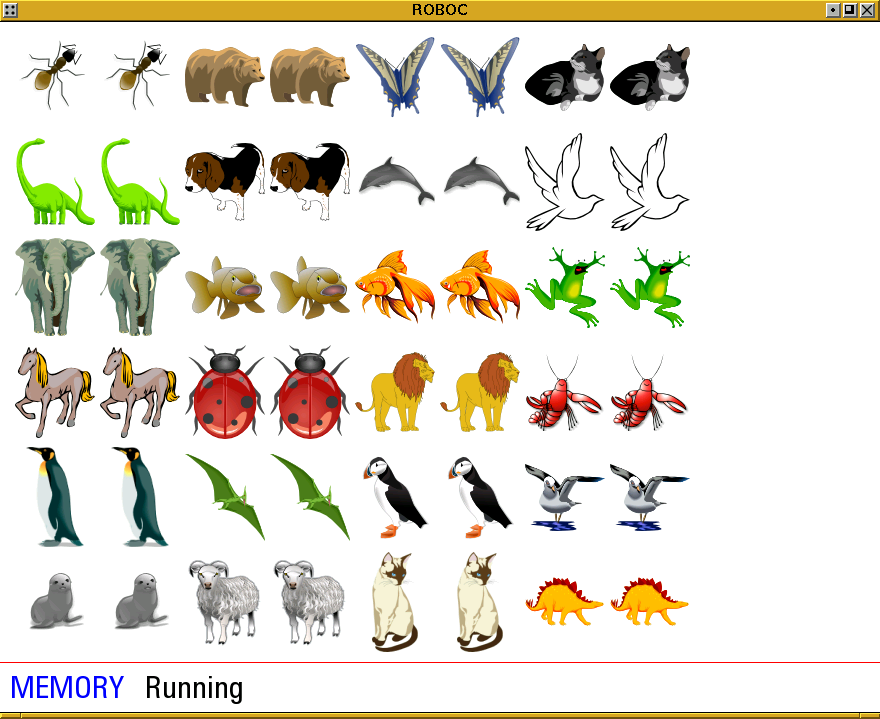
\includegraphics[scale=0.32,angle=0]{screenshots/artpixel/memory/animal_grid}
% 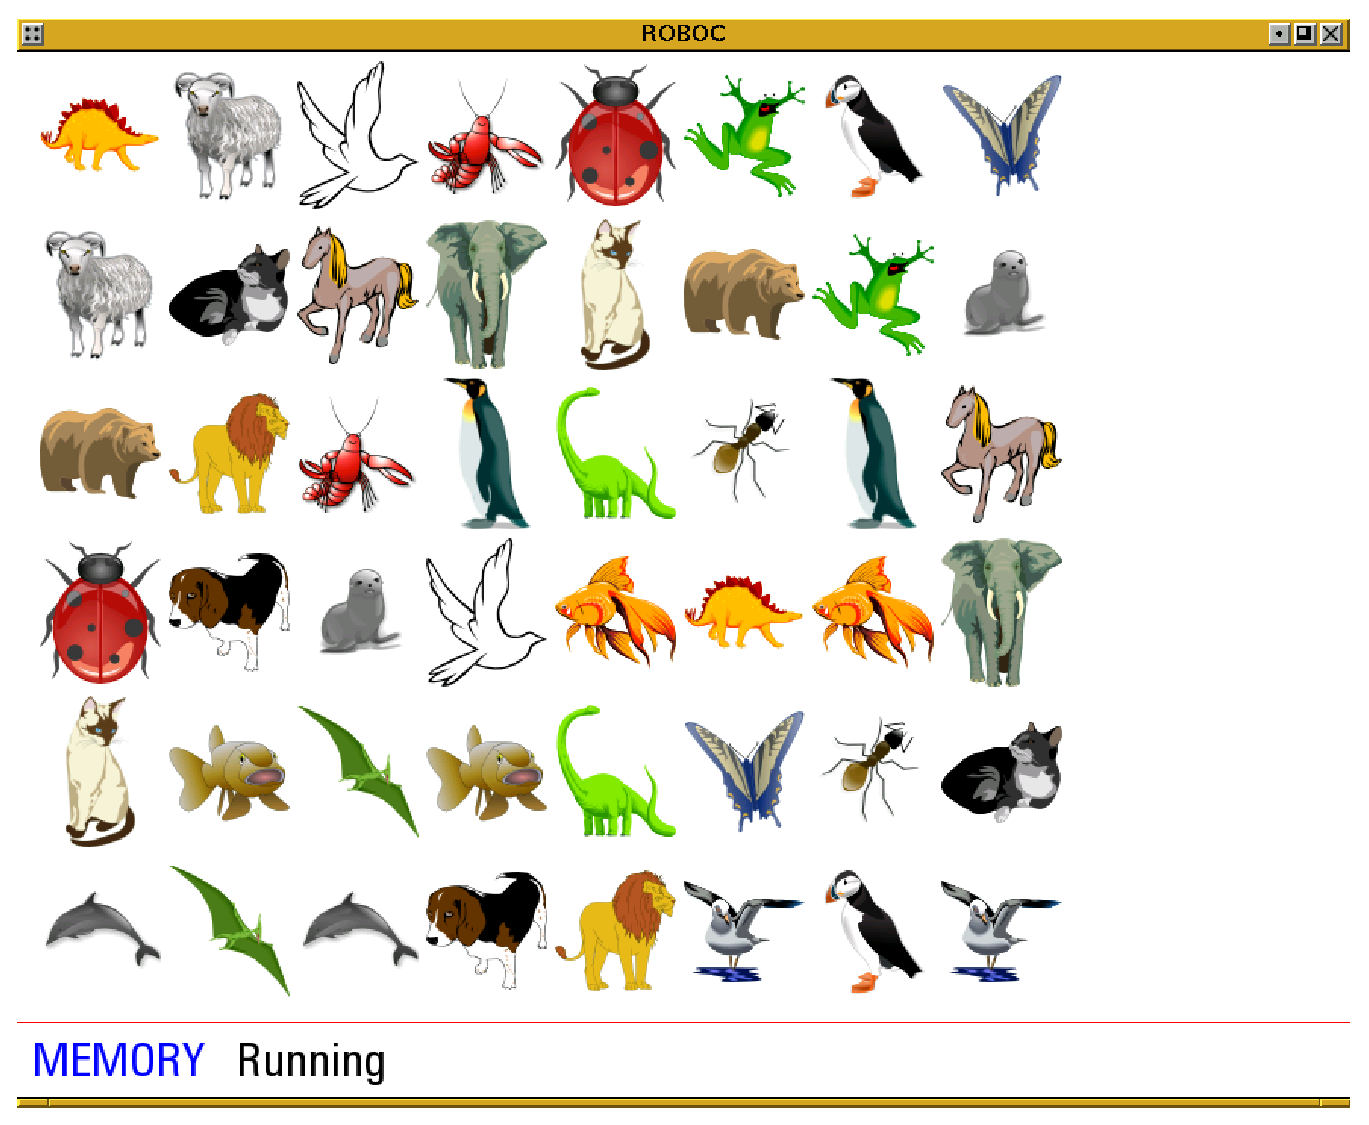
\includegraphics[scale=0.32,angle=0]{screenshots/artpixel/memory/animal_random.eps}\\
% 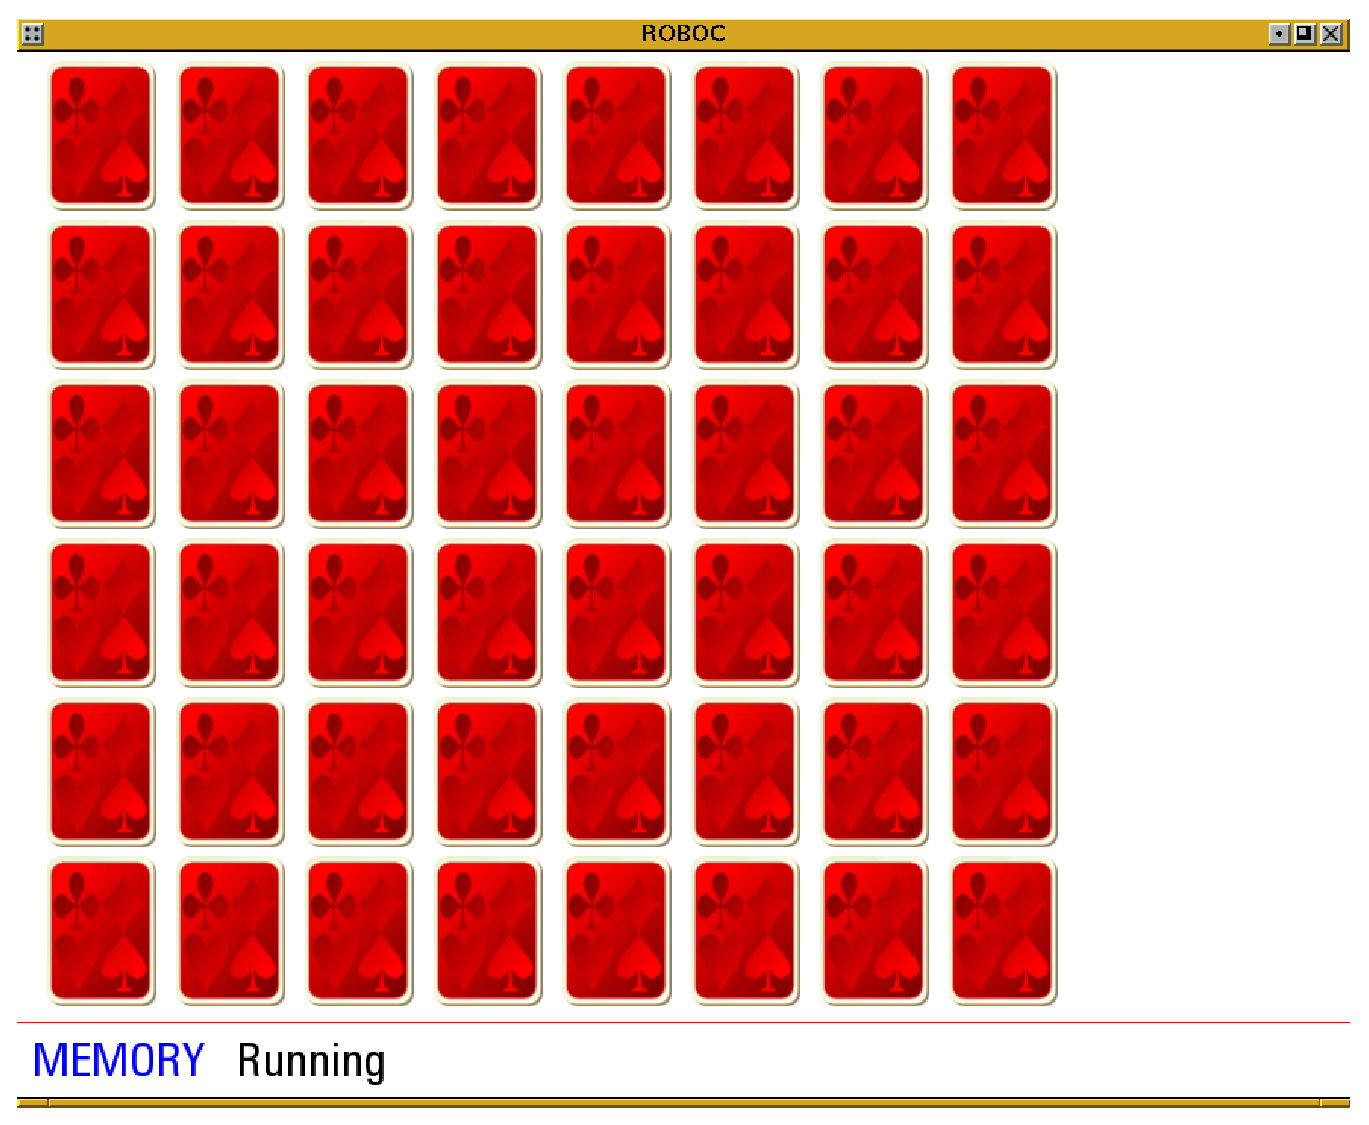
\includegraphics[scale=0.32,angle=0]{screenshots/artpixel/memory/card_backs.eps}
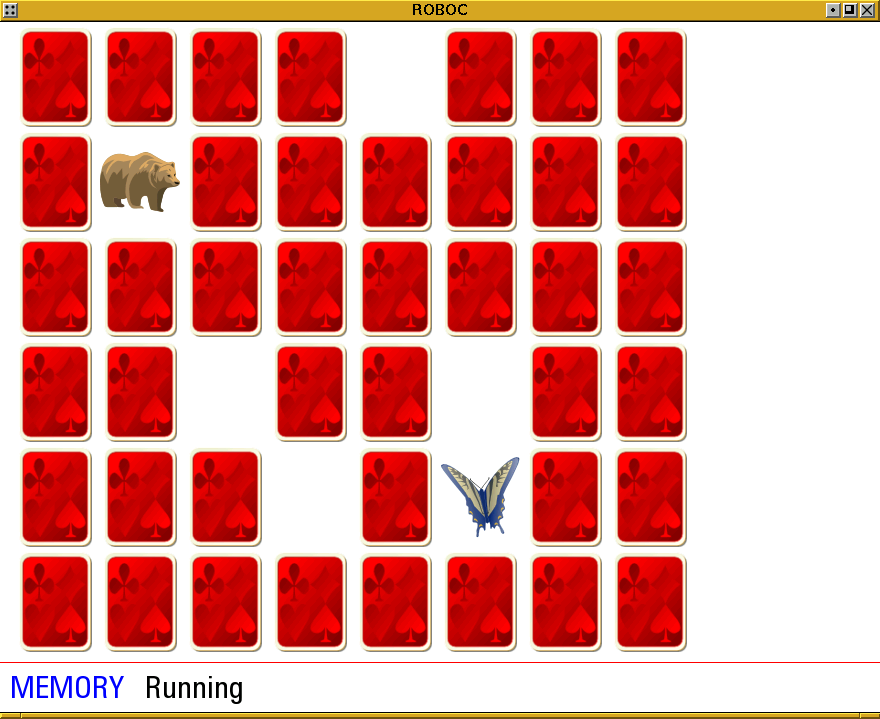
\includegraphics[scale=0.32,angle=0]{screenshots/artpixel/memory/playing}\\
% \begin{center}
% 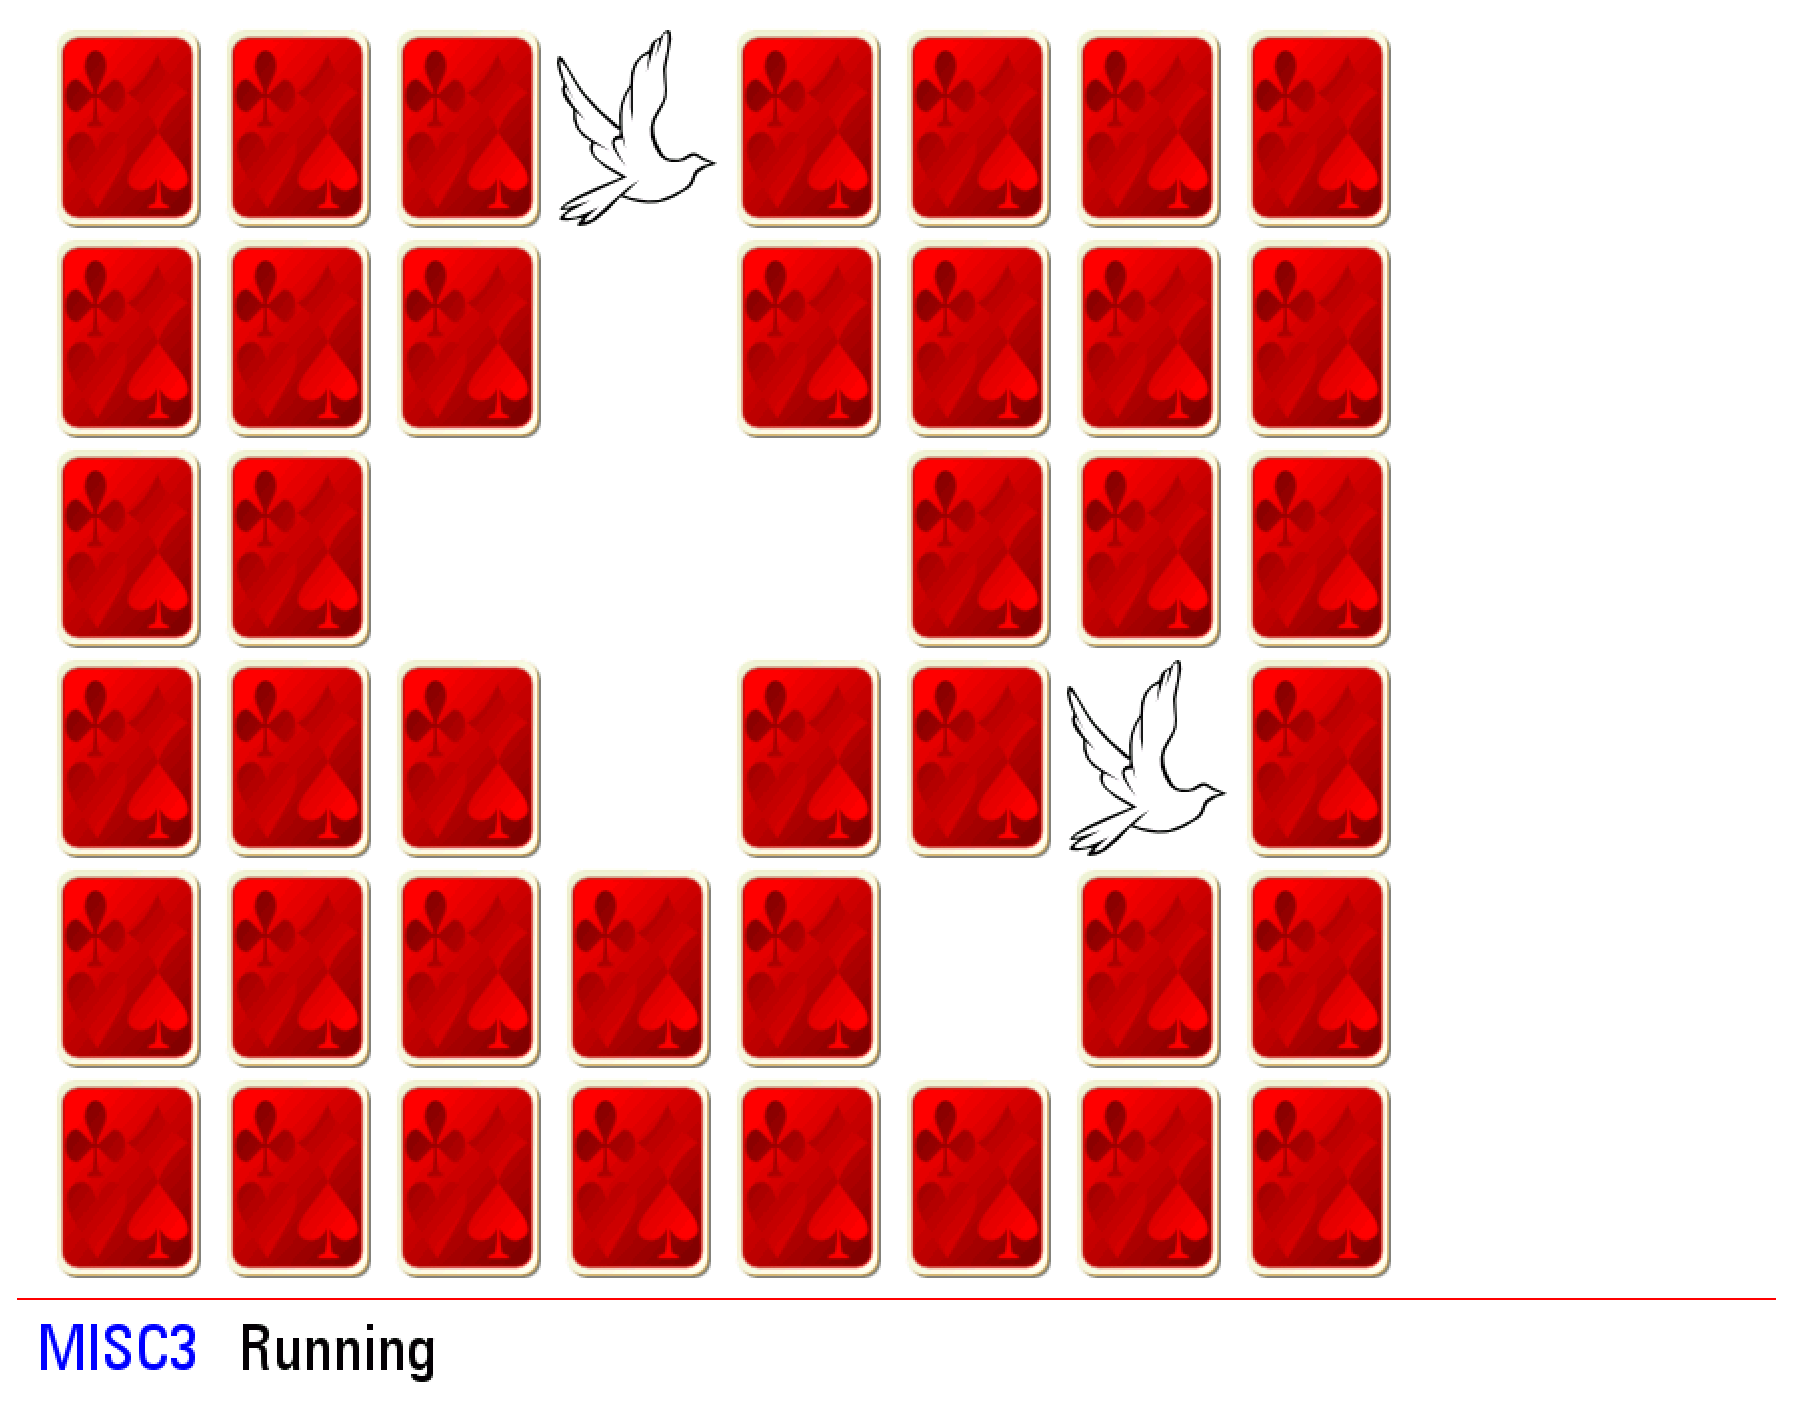
\includegraphics[scale=0.25,angle=0]{screenshots/artpixel/memory/snap.eps}
% \end{center}
\end{center}

\newpage
\section{Racetrack \it{(Hard)}}

This project develops a simple car racing game. Start by calling
\verb^background "track"^ to display a racetrack. Now write a function
to display a small car somewhere on the track. To keep things simple
we are going to use a triangular car, like this:

\begin{center}
%\fbox{
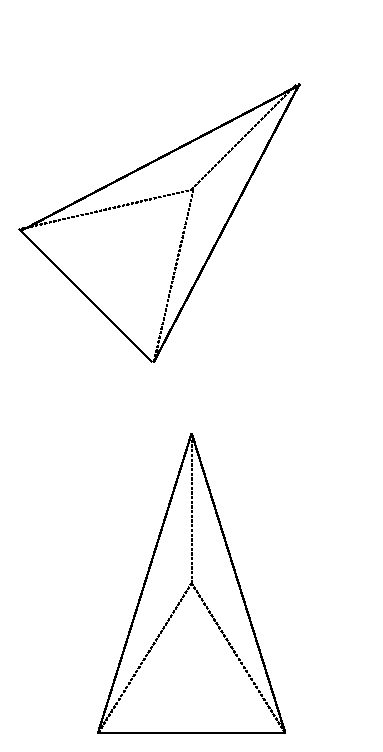
\includegraphics[scale=0.32,angle=-90,trim=20mm 20mm 145mm 140mm]{diagrams/car}
%}
\end{center}

The dotted lines give you an idea of how to calculate the positions
of the corners from the centre point. You will have to use \verb^sin^ and
\verb^cos^ functions of the appropriate angles. Once you have worked out
the positions of the corners, connect them with lines using the \verb^line^
function. Now create a function which can draw the car at any position
and facing in any direction, using parameters.

See the Events section of the user manual and make your car respond to key pressed. Respond
to the left and right arrow keys by spinning the car anticlockwise
or clockwise. When the car's direction changes you will
need to erase the old car (by drawing it again but in white), then
call the draw function again with a different angle in the colour of the car.

Next add an accelerator key, and a key for reverse gear (only operable
from stationary). When the accelerator is pressed, the car should
speed up (create a variable to keep track of the current speed).
When the accelerator is not pressed, it should slow down gradually.
Again you will need to do some trigonometry based on the direction it
is facing to work out how to update its position.

\subsection{Extension}

Make this into a two-player game. First use a single computer with
different control keys for the second player, then use the networking
feature to have the players on different computers. See the extension
to the Paint Program for some suggestions on how to make this work.

%A further extension would be to add a "trigger" button which allows
%the cars to shoot at each other. You will need to think about simulating
%the position of the bullets and detecting collisions with the other cars.

%Yet another extension would be to make this game support a larger number
%of players, all on their own computers.

\newpage
\section{Minesweeper \it{(Medium)}}

This project is to create a Minesweper clone in Tealight. The game consists of a
grid of squares. Each square either contains a mine, or a number stating how
many mines there are in the 8 squares around the current one.  Initially all
squares are covered. The player then has to click squares: left click to
uncover the square, right click to mark the square as a mine.  Once all the
non-mine squares are uncovered, the player wins; if the player uncovers a mine,
they lose.

Consider how you would store the two-dimensional game grid as a one-dimensional
array. Each square's value will be represented as either the integer number of
mines around it, or \verb^-1^ for the mines themselves. You will also want a
second array to remember which squares are uncovered. You can use the values
\verb^0^, \verb^1^ and \verb^2^ to represent "covered", "uncovered" and
"marked". You can make the grid be 10x10.

First, write a function \verb^draw^ which draws the game grid. Use \verb^print^
to draw the numbers, draw mines as red spots and marked squares as blue spots.
You may find it useful to write \verb^get(x,y)^ and \verb^set(x,y,value)^
functions to get and set the value of a coordinate in the grid.

Initially, your grid will be empty. So, write a function \verb^init^ which adds
15 mines to the grid, in random positions, and then calculates for each
non-mine square how many mines there around it. When testing this, you may find
it convenient to show all entries in the grid as uncovered.

Then, you can start your game loop. Write a loop which listens for mouse
clicks, using \verb^input()^. For each mouse click, calculate which element in
the grid the player clicked on, and set the "covered" or "marked" state
appropriately. If the player uncovered a mine, display a "Lose" message and (on
the next click) restart the game using your \verb^init^ function. If the player
has uncovered all the non-mine squares, display a "Win" message and restart the
game. At the end of the loop, call your \verb^draw^ function.

\subsection{Extension \it{(Hard)}}

In the real Minesweeper game, clicking on a 0 square (one with no mines
surrounding it) will uncover that entire "island"; that is, that entire
connected region of 0 squares, plus the surrounding numbered squares. Make your
clone do the same thing. You may have to write a recursive \verb^uncover^
function which, for 0 squares, call itself on all the neighbouring squares.

\newpage
\section{Othello \it{(Medium)}}
This project involves creating the game of "Othello" (also known as "Reversi").

Othello is a two-player game. Players take it in turns to place coloured
counters on a board. If a player arranges for their own colour counters
to be at both ends of a row of counters (horizontal, vertical or diagonal),
all the counters in between change to that colour. The object of the game 
is to turn all the counters into your own colour.

Start by constructing an 8x8 game board. When you click on a cell, a
coloured spot should be drawn in the cell. Arrange it so that the colour
of the spot alternates with each click.

You will probably want to represent the game board in an array, with each
cell storing whether it is empty or has a counter in it. Players are only 
allowed to place counters next to other counters, so you will need to add this
restriction. At the start of the game, there are four counters on the board:

\begin{center}
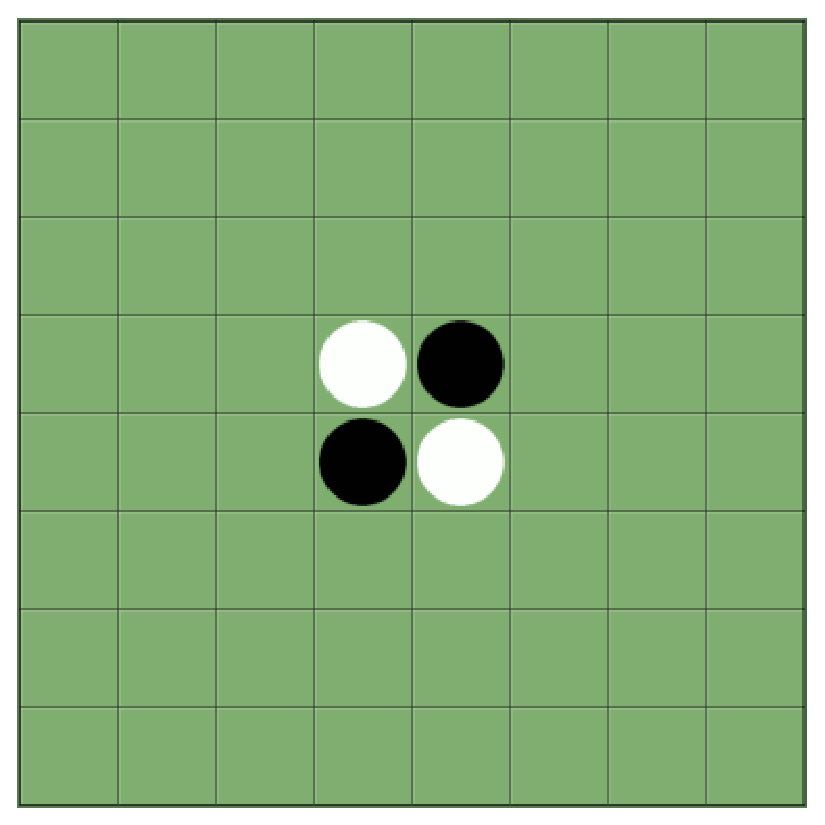
\includegraphics[scale=0.6,angle=0]{screenshots/othello}
\end{center}

The game ends when all the counters are one colour, or there are no spare
spaces to add counters.

\subsection{Extension}

Add networking to the game, so that the two players can be on different
computers. See the extension of the Paint program for some suggestions.



\newpage
\section{Lights Out \it{(Easy)}}
This project is to create the game of "Lights Out". This is a single-player
game which consists of a 5x5 grid of lights. When the game starts, a random
selection of lights is switched on. Clicking any light will toggle it and the
four adjacent lights. The goal of the puzzle is to switch all the lights off
in as few button-presses as possible. The image below illustrates the game-play.

Have a look at the Minesweeper and Connect4 projects for hints on storing the
state of the lights.

\begin{center}
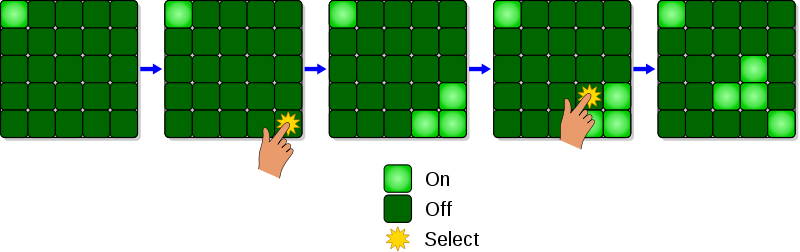
\includegraphics[scale=0.6,angle=0]{screenshots/lightsout}
\end{center}



\newpage
\section{Connect 4 \it{(Medium)}}

This project involves creating a game of connect 4, where the object of the game
involves creating horizontal, vertical and diagonal lines of 4 counters in the
same colour on a grid. Players take it in turns to place their counters, both
trying to block the opponent from creating lines whilst trying to create their
own.

A simple starting point would be to create an 8 by 8 grid, and allow the players
to place their counters. You could use an array to store which counters are placed
where. Using that array you can then add the logic that checks for lines of 4
counters and display the winner. The game should also display whose current turn 
it is during the game.

\subsection{Extension \it{(Medium - Hard)}}

The scoring could be changed to allow lines longer than 4, which would be worth 
more points, however the size of the grid should be increased to accomodate this.

You could also add special squares, chosen at random, where if you place a counter
you get a bonus - an extra go or a bomb to remove a counter of the opponent.

Connect 4 is usually played on a table in an upright frame - add gravity to your
grid, so counters appear in next avalible slot, and have the user only able to
select collumns.

Animate the counters being placed, as they drop down into their slots - you could
also add a winning animation where all the counters fall out of the board at the
end.

Finally, you could add networking support to enable players on different computers
to compete. This could also allow many more than two players, each with their own 
colour counter, and a much bigger grid!

%% Removed for 2013 - Lots of groups did this in 2012 and they really weren't that good. 
%\newpage
%\section{Virtual Pet \it{(Hard)}}
%The aim of this project is to develop a digital pet. The pet should be 
semi-autonomous - it should have a life of its own, but also respond 
and depend on the owner (player). At the very basic level, your pet should 
be able to fall asleep when tired and need to be fed, but there is no limit 
to what else you can add (playing with a pet, pet getting 
ill, having multiple pets, etc.). For more inspiration, check the article 
on Tamagotchi in Wikipedia.

To start with, you should have two simple counters (for tiredness and hunger),
which should slowly be incremented over time, and reduced when the pet 
sleeps or eats. Your program should have buttons for interacting with the 
pet (feeding it, playing with it, etc.) and respond to them appropriately 
(update the counters, show animation, etc.). As an extension, you could 
consider how different levels of counters can interact with each other 
(e.g. maybe if the pet is hungry, it does not want to play?).


%\newpage
%\section{Robot navigation}
%
%In this project you will write a program to control an iRobot Create
%robot and help it navigate around the floor of the room. The robot
%is connected to a OLPC laptop which provides remote control from
%ROBOC. Human control
%is not allowed, so your program must steer around obstacles itself.
%You should run in Art mode but it is not necessary to draw anything
%on the screen.
%
%To control the robot, send network messages to the user \verb^robot^.
%Each message must contain a single letter; this can be \verb^a^
%to accelerate the robot forward, \verb^d^ to decelerate it,
%\verb^l^ to make it turn to the left or \verb^r^ to make it turn
%to the right. Two or three accelerates in a row will make it move faster.
%A message containing \verb^s^ can be used as an emergency
%start/stop from any speed.
%
%To find out if the robot has hit an obstacle, make sure your
%program includes\\
%\verb^self("controller")^\\
%You can then listen
%to \verb^NetEvent^ to receive collision messages. These will
%consist of either the letter \verb^L^ or \verb^R^ to indicate
%a crash on the left or right side of the robot's front
%bumper respectively. Make sure you tell the robot to stop
%immediately when it has had a collision!
%
%Your program should help your robot explore the area by diverting
%around objects in its path. During the project presentations you
%will be given a maze you have never seen before and the robot
%must get through it. The robot will always be positioned so that
%it starts facing directly torwards the goal and at a distance
%of exactly 5 metres, however.
%
%You may find it useful to keep
%track of time with the Art mode \verb^delay()^ and \verb^time()^
%functions, and work out how fast the robot travels and what
%angle it rotates by when turning on the spot. These can
%help you calculate how to get the robot back on target after
%it has to divert to avoid an obstacle.
%
%\newpage
%\section{3D pinball}
%
%This project is done in 3D mode, instead of Art mode.
%First create a rectangular pinball table with a moving ball
%on top of it. The ball's X and Y co-ordinates and
%horizontal and vertical speed need to be kept in global
%variables so that they are not reset each time the program
%runs to redraw the 3D scene. Hint: if you want to set some initial
%values for them, use another variable called \verb^setup^ which
%is initially 0 but gets set to 1 after the first run.
%
%Make the ball bounce off the four edges of the pinball table
%by reversing its velocity in the appropriate direction when it
%reaches the edge. Now
%tip the table by rotating about the X axis by 30 degrees,
%and program keyboard controls
%to adjust the tilt (say the 9 and 0 keys). You will need to
%listen to \verb^KeyPress^ events and use the \verb^poll()^
%function. Add gravity, the strength of which will depend on the current
%angle of the table. The effect of gravity is always to accelerate
%the ball down the Y axis. Also add some friction
%which gradually reduces the ball's Y-axis speed over time.
%
%Next make the 1 and 2 keys control two large flippers at the
%bottom of the table. These should move when the relevant
%key is pressed and return when it is released (using
%\verb^KeyRelease^). If the ball is near to the flipper when
%it moves it should be accelerated along the Y axis.
%
%Now consider obstacles for the ball to bounce off in
%the middle of the table. Can you create a row of bricks stored in
%an array, which
%disappear when the ball hits them, like in Breakout?

%\newpage
%\section{Shared whiteboard}
%
%This project is to allow two users on different computers to participate
%by drawing on the same canvas (so both users see the results of both
%drawing on their screen). You should start with the sketch program,
%and add networking. First use the \verb^send^ command to notify the other
%computer when the user has clicked with the mouse. The other program
%should add \verb^NetEvent^ to the event types it is listening to.
%Initially you might arrange for it to display a shape in the
%corner of the screen when the other user clicks with the mouse, just to
%test the communication is working. Make it work in both directions.
%
%Next you will need to encode the coordinates where the other user has
%clicked within the network message it sends. You can use the string
%join operator (\verb^:^) to do this, and the \verb^word(n, string)^
%function at the other end to extract the information. If a text string
%consists of just a number it is automatically converted to numeric form.
%If the basic program works, can you encode the difference between
%clicks and drags, or which mouse button was used?
%
%This project only requires a short program to solve, but a significant
%practical difficulty is making sure the programs on the two machines
%you are using are kept up to date, and do the same things (there is
%no automatic way to transfer a program to another computer).

% \section{Map tool}
%\newpage
%\ 
%\newpage
%\section{Project preferences form}
%
%{\Large
%Name:\\[1mm]
%
%Username:\\[1mm]
%
%Previous programming experience:\\[10mm]
%
%1st choice:\\[1mm]
%
%2nd choice:\\[1mm]
%
%3rd choice:\\[1mm]
%}

\end{document}
